\section{Solution}\label{solution}

Our goal with the migration to an SPL is to switch the mindset from `my project'
to `one of our product variants' by enabling the software teams to collaborate
in a single Git repository and be able to use all variants in a single IDE
instance to build any target of any product variant. Our SPL implementation uses
Visual Studio Code plus CMake Tools extension as IDE, CMake and Ninja for
building all required targets, Powershell and Python as build wrapper and CI/CD
test runners.

With the help of our SPL implementation we follow a migration strategy that
consists of three consecutive steps as depicted in Figure~\ref{fig:migrationFlow}.

\begin{figure}[htb]
  \centering
  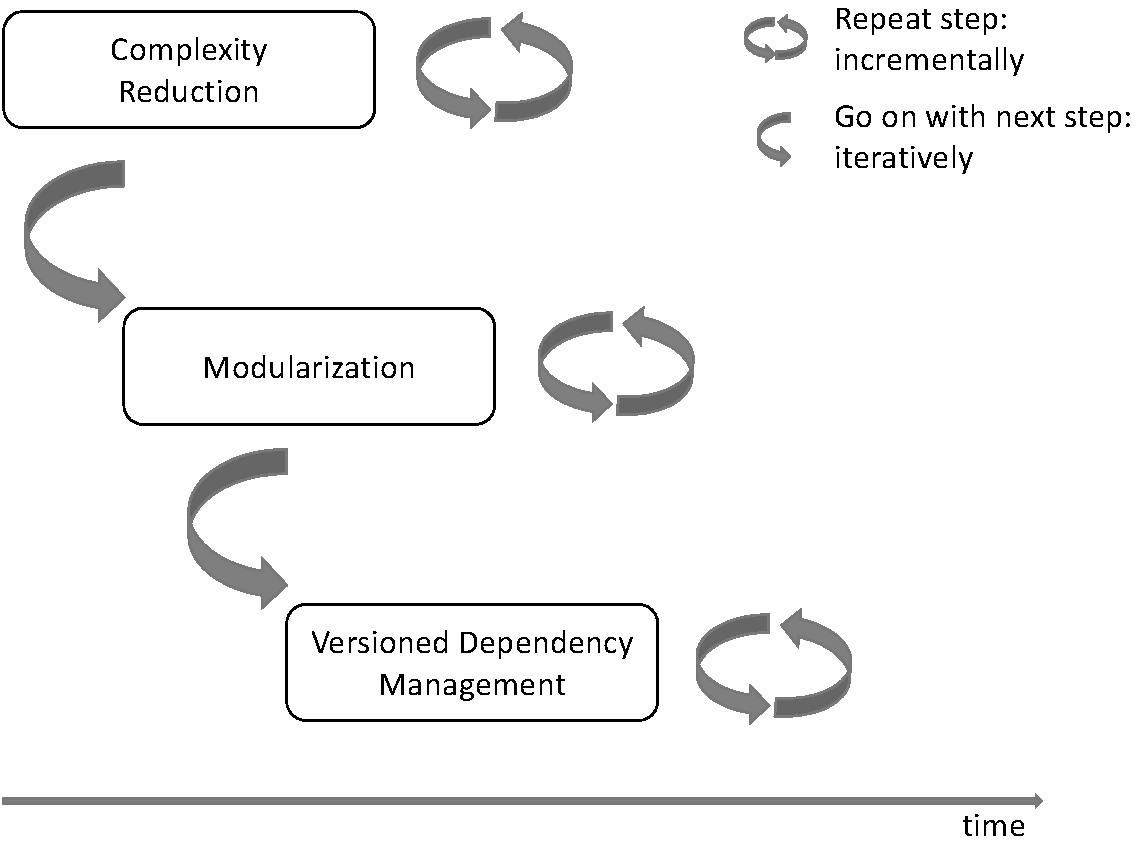
\includegraphics[width=1\columnwidth]{migration-steps-overview.pdf}
  \caption{Migration Flow Overview}
  \Description{Migration Flow Overview showing the three proposed migration steps}
  \label{fig:migrationFlow}
\end{figure}

In an SPL we talk about at least two variation dimensions: space,
time~\cite{appliedSPLE} and sometimes also maturity~\cite{bigleverwhitepaper}.
Our first migration step \textit{Complexity Reduction} is merely a step to
prepare these dimensions, to bring code together that belongs together within a
new SPL-capable build system. The second step \textit{Modularization} enhances
the space dimension by building up configurable sources or variants of software
components to reduce lines of code and maximize reuse. With variation in space
we are able to create feature variants of our software and its components and
this is the beginning of the SPL idea. The third step \textit{Versioned
Dependency Management} focuses the time dimension and cross-product component
reuse.

All three steps will be explained in detail in the following subsections.
It is important to know though, that each step can be done incrementally:
\begin{itemize}
  \item \textit{Complexity Reduction}: variant by variant.
  \item \textit{Modularization}: component by component.
  \item \textit{Versioned Dependency Management}: component by component.
\end{itemize}

If one step is accomplished for a variant or a component, the migration of that
specific variant or component can iteratively proceed with the next migration
step.

The content of the SPL repository, especially the number of lines of code (LOC),
will change during the different migration steps as shown in
Figure~\ref{fig:threeMigrationSteps}. In the first migration step
\textit{Complexity Reduction} the LOC will increase with every legacy project
added to the codebase. During \textit{Modularization} legacy sources will be
exchanged with configurable sources leading to a reduction of duplicated code
and therefore to a decreased LOC.\@ Finally even the LOC of configurable sources
in the SPL repository will decrease, as the sources are isolated and moved to a
separate repository during the third step \textit{Versioned Dependency
Management}. Then those configurable sources will just be configured as external
build dependencies in several product families.

\begin{figure*}[ht]
  \centering
  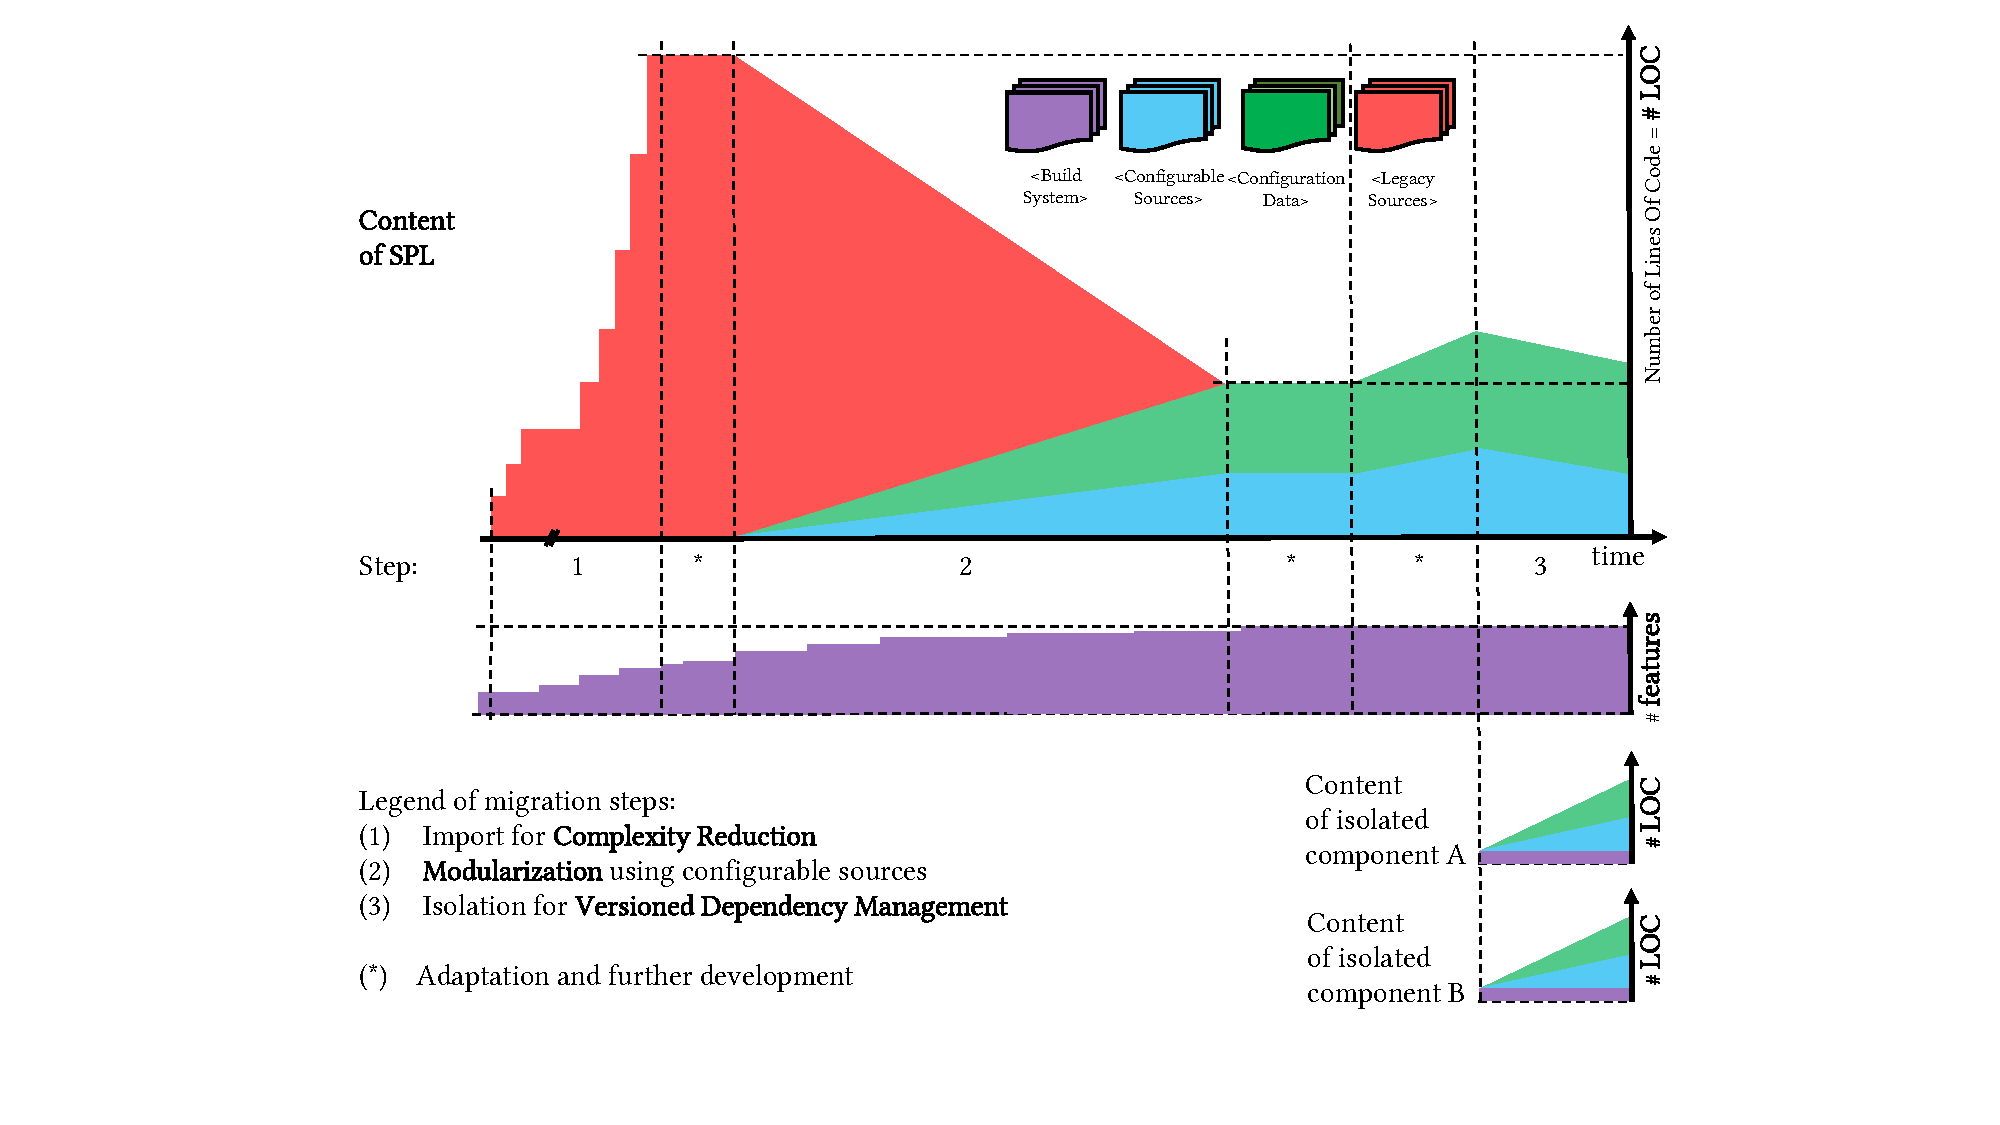
\includegraphics[width=1.65\columnwidth]{migration_steps.pdf}
  \caption{Three Migration Steps to SPL}
  \Description{Three Migration Steps to SPL}
  \label{fig:threeMigrationSteps}
\end{figure*}

\subsection{Complexity Reduction}\label{complexity}

Our first step towards SPL consists of importing several active sensor projects
into the SPL, i.e., adding Dimension rdepository product variants into one
structured Git repository. To support further incremental imports of additional
sensor variants we implemented a tool called
Transformer~\cite{GithubTransformer} that highly automates the necessary import
steps. The Transformer is implemented in Python and can be applied to each
variant separately, therefore making the transformation incremental and
independent of already existing or upcoming variants. The transformation of a
legacy project into a new product variant is divided into four parts:

\begin{enumerate}
  \item \textbf{Copy sources}: The variant's original source tree is copied
        into a variant-specific legacy tree without any further changes or
        adaptions.
  \item \textbf{Create build configuration}: The original project build
        system (GNU Make) is used to extract all variant-specific configuration and
        to transform it into a CMake configuration and part list compatible with
        the SPL build system.
  \item \textbf{Create IDE configuration}: For seamless integration of the SPL
        repository and its variant concept into Visual Studio Code the
        CMake Tools extension is used. This extension introduces the concept of CMake
        Variants, therefore we create a configuration file with build settings
        for each variant.
  \item \textbf{Establish CI/CD}: In order to simplify the switch to the new
        tool environment, introduce a CI/CD system to increase automation and
        validation for every source code change.
\end{enumerate}

Switching from variant-specific repositories in Dimensions to a single Git
repository in Bitbucket causes a high workflow impact for the developers.
Additionally they need to get used to an SPL build system and a new IDE.\@
Therefore, we decided not to change the production source code during this first
migration step so that the developers can continue to work in their well-known
code basis.

The DevOps Handbook~\cite{devopshandbook} calls this a monolithic approach and
positively emphasizes the simplicity and resource efficiency in small scale. It
also mentions the drawbacks of overall poor scaling and weak modularization
capabilities. We are aware of those drawbacks and are going to tackle them
within the third migration step \textit{Versioned Dependency Management}.

The structure after the transformation looks like this:
\begin{Verbatim}[frame=single,samepage=true]
.vscode/
  cmake-kits.json
  cmake-variants.json
  settings.json
legacy/
  variant-a/
    component-1/
    component-2/
  variant-b/
    component-1/
variants/
  variant-a/
    config.cmake
    parts.cmake
  variant-b/
    config.cmake
    parts.cmake
CMakeLists.txt
\end{Verbatim}

The `legacy' folder contains all the projects' unmodified source code in
variant-specific folders. The configuration and part lists of the variants can
be found in the `variants' folder.

Although the build system and tool environment is reused already for all
variants, for source code there is no reuse in place and the LOC is growing over
time as shown in Figure~\ref{fig:threeMigrationSteps}, therefore scaling may
become problematic. Still there are a lot of advantages with the monolithic way,
like centralized deployment with our CI/CD system, start learning to use Git as
source code management system and reducing complexity by reducing the number of
systems: polyrepo vs.\ monorepo with a single build system and tool environment.

\subsection{Modularization}\label{modularization}

As soon as all developers, software project managers and integrators are used to
the outcome of the first step of the SPL migration, the \textit{Modularization}
step can begin. With the following three stages it is possible to switch from a
project to a product perspective. The goal is to merge the legacy sources into
configurable sources, keeping variant-specific functionality, to maximize reuse
and reduce maintenance effort. Thinking in terms of products rather than
projects helps to reduce the LOC and maximizes the reuse across all variants. In
order to build up software components, consisting of core assets and
variant-specific functionalities, a feature model is required for configuring
the software and thus controlling the execution flow. Although CMake is capable
of handling very simple feature models with variables and template generators
pretty well, a more complex feature model might require another tool to manage
it. Our recommendation for complex feature model configurations is KConfig, `a
domain specific language designed specifically for coding the Linux kernel
variability model'~\cite[page 3]{kconfigKernel}. KConfig is able to manage the
complex design of the Linux kernel and it has enough functionality to work with
most embedded applications. Additionally it is open-source and free to use for
anyone. Alternative solutions might also fulfill the configuration purpose.
Prominent examples are pure:variants~\cite{pureVariantsPureSystems} from pure
systems or Gears from BigLever~\cite{gearsBigLever}. Both tools are known to be
highly flexible and easy to integrate into existing
projects~\cite{confsplcGrunerBKR20}.

Independent of the feature model tool the modularization process should be the
same. All stages of the \textit{Modularization} step are visible in
Figure~\ref{fig:step2Modularization} and will be further described in detail.

\textbf{Migrate from legacy component to product component:} After the first
step \textit{Complexity Reduction}, all source code files are located in a
dedicated legacy folder. This legacy folder contains a folder for each
variant, holding all software components separately. Using a component in
multiple variants is possible, but does not make much sense. There is no reason
to share the variant component variant-a/component-1 also in variant-b. In this
step, components are just moved into a generic source folder. The folder
structure will change from:
\begin{Verbatim}[frame=single,samepage=true]
legacy/
  variant-a/
    component-1/
    component-2/
  variant-b/
    component-1/
\end{Verbatim}
to:
\begin{Verbatim}[frame=single,samepage=true]
src/
  component-1/
    variant-a/
    variant-b/
  component-2/
    variant-a/
\end{Verbatim}
By doing this, all variants of one component, with the identical or very similar
functionality, are moved to the same folder. Variants of a component residing
next to each other are easier to compare and to handle. This will enable reuse
already, but without the following stages it has no positive effect on LOC
reduction or maintenance effort.

\textbf{Remove duplicates and derive core assets:} Within the new structure
established in the previous stage, we recommend to clean up duplicate variants.
Variants of a component are considered as duplicates if their source code is
identical and no configuration is required. This is a fast and easy step for
reuse and will not require additional knowledge about a feature model or the
functionality. Removing duplicates is followed by separating core assets and
variant-specific functionality with a decorator pattern. The separation can be
done on a function level and requires static function interface definitions. The
concept is to create:
\begin{itemize}
  \item a core asset C file, which contains generic code across all variants,
        considered to be static,
  \item a header file with interface descriptions of core assets and decorators,
  \item a decorator C file for every variant, which contains a variant-specific
        implementation of a function; the function signature must be identical
        for all variants and shall be defined in the according header file.
\end{itemize}
This way the core assets and the decorators can be developed without any need of
conditional compiler directives. It is possible to implement variant-specific
differences in an object-oriented manner in C. The idea is to provide a
product-specific core asset and additionally one interface with multiple
variant-specific decorators that extend the shared functionality. The feature
model's responsibility is to take control of the underlying build system and
configure the correct decorators. If a separation of core assets and
decorators in individual files is not possible or not wanted for any reason,
another option would be to use a feature configuration with conditional
preprocessor directives or runtime configuration. Toggle points in the code make
it possible to select different implementations within the same C file.

\textbf{Refactor with focus on variability:} Last but not least, the code should
be refactored according to variability. This is the first stage that has a
functional impact on the code, and it requires a mindset change. One must stop
thinking about project-specific features and define component-specific features
relevant for the product family. Most of the legacy components do not support
variability and might require substantial refactoring to have a meaningful
feature set.

We highly encourage to implement unit tests before the refactoring starts, if
there are no unit tests available already. Refactoring can have effects on the
compiled binaries and change the behavior, even though it was not intended by
the developer. A feature model will generate many possibilities to configure the
software, therefore unit tests covering all core assets and features will ensure
that no functionality was broken and will reduce time in finding errors at a
later development phase.

\begin{figure}[htb]
  \centering
  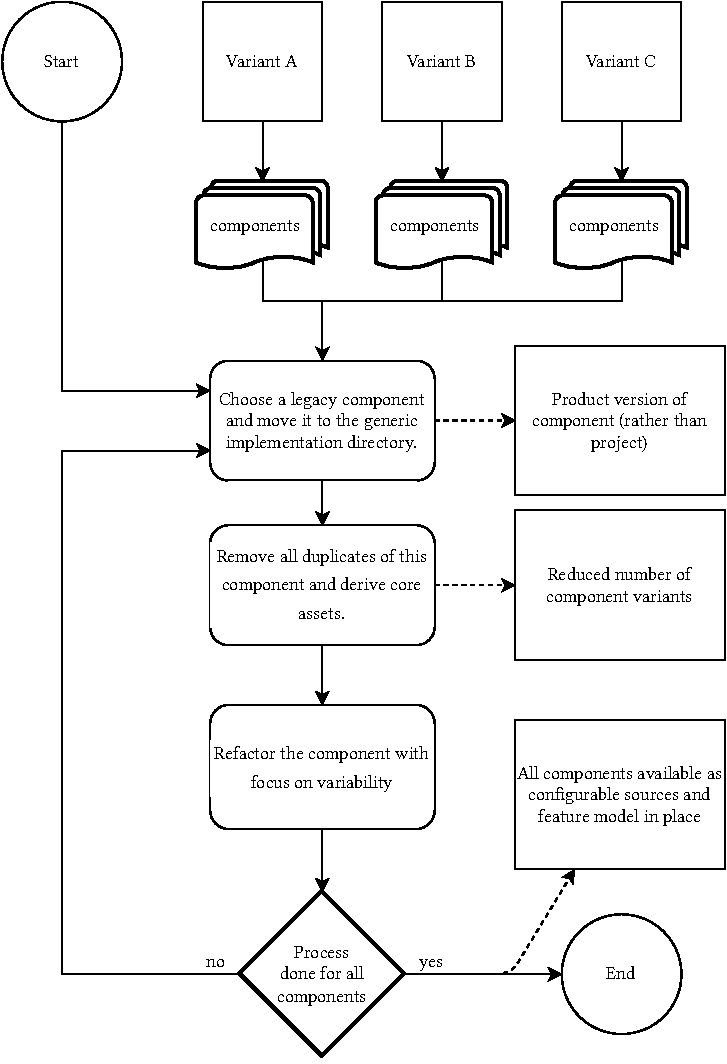
\includegraphics[width=1.0\columnwidth]{step2-modularization-flow.pdf}
  \caption{Detailed stages of the \textit{Modularization} step}
  \Description{Detailed stages of the Modularization step.}
  \label{fig:step2Modularization}
\end{figure}

\subsection{Versioned Dependency Management}\label{dependencies}

The first two migration steps focused on the space dimension, how to organize
the source code using components and variants. This step deals with the time
dimension. By using Git it is already possible to get a variation in time. At
any created commit, it is possible to create a new branch. This branch can be
the active development branch with all the latest changes, or it can be based on
a former commit to represent a baseline of the SPL that is going to be released
or was released already. If bug fixes are required after a release, they will be
done on the same release branch. With this strategy, releases can be done on a
stable code basis without the influence of new feature developments of other
branches. Additionally the documentation of release relevant changes becomes
simple. The release branch will stay unchanged and usually not get any feature
updates, but only fixes. But release branches in a monorepo come with some
drawbacks. It is complicated to get different versions of different components.
A baseline must be done on the entire software. An integration of mixed versions
is possible but requires lots of manual effort and will likely have a strong
negative impact on maintenance. Adding a fix in a component of a specific
version in a release branch will not become available in the same version of the
same component in any other branch. All commits and branches are independent of
each other, so no automatic reuse of code between them is available. Therefore
using the same component and version provides no reuse in the space dimension if
we introduce the time dimension like this. And finally fixing a bug in a new
version, that was spotted in an earlier version, is even more complicated,
especially across all branches. Our proposal requires some more changes to the
build system and infrastructure. It is required to split up the repository
again. With the modularization being done, the split will not be done per
project anymore, but per software component. Each modularized software component
will reside in its own repository and is maintained separately. This allows us
to work with different developers or development teams on different software
components independently. To enable the development of a software component in
its own repository the following requirements must be fulfilled:
\begin{itemize}
  \item component specific requirements specifications,
  \item mocked required interfaces,
  \item unit tests for all component features in all possible configurations,
  \item software integration tests and
  \item a software test plan.
\end{itemize}
Although this step introduces a polyrepo workflow it still follows the SPL
concept by dividing products into smaller pieces still developed in SPL
repositories. The SPL repositories of the products do not contain the sources of
the isolated components anymore but each SPL repository has dependencies to
specific versions (baselines) and variants of the isolated components. These
dependencies might be references to commits of a Git repository or to released
component package artifacts, e.g., with JFrog Conan.io. This step can be done
incrementally again, component by component. The SPL repository's build system
will then do the integration job. With a proper dependency management, the build
system will integrate requested software components from external repositories
of any kind and configure them according to the feature model of the selected
variant. The benefits of this approach are the following:
\begin{itemize}
  \item Components are being developed and tested independently to get a faster
        release loop.
  \item A fix of a buggy version is implemented only once in the component's
        repository.
  \item Buggy versions can be marked in the components' repositories. With this
        variant builds containing a buggy version can print a warning or error.
        The integrator can then manually update the version of the dependency or
        justify the warning in regards to their project setup. An automatic
        update would also be possible.
\end{itemize}
Since all components are being developed independently, one package version
might not be compatible with another component's package. With Conan.io
`compatibility can even be configured and customized on a per-package
basis'~\cite{conandocs}. This is why we recommend Conan.io over Git submodules
or similar techniques. The development team together with their integrators can
configure this compatibility check. An AUTOSAR architecture might make this
check easier. An application software component should only have interfaces to
the Run-Time Environment (RTE), so based on the RTE configuration a
compatibility between components should be clearly defined.

\textbf{Cross-product component reuse:} Independent of an SPL introduction, it
is most likely that within the product portfolio of an automotive supplier like
the Marquardt GmbH with a wide range of different products, those products share
similar components and solutions. When such a company applies SPL engineering
for one of its products, sooner or later the concept is taken over for other
products of other business units, too. In case the second step of SPL migration
\textit{Modularization} is finished in at least two SPL repositories with
similar core assets and step three has been performed on a few components, the
probability, that the need to share those components between the different SPL
repositories will arise, is rather high. Therefore the third step of our
migration concept provides an additional useful feature: isolation of
configurable sources for \textit{Cross-product component reuse}. The idea is
that the isolated software component and all its variants can be used in
multiple other SPL repositories, not just in one. There are functionalities,
e.g., current or voltage measurement, that might be useful in a multitude of
electronic products. This can exponentially increase reuse in the entire product
portfolio.
